% !TeX spellcheck = en_US
\documentclass[letterpaper]{article}
\usepackage[utf8]{inputenc}
\usepackage[spanish, mexico]{babel}
\usepackage{amssymb, amsmath}
\usepackage{stackengine}
\usepackage{graphicx}
\usepackage{ mathrsfs }
\usepackage{lipsum}
\usepackage{dsfont}
\usepackage[margin=1.5cm,
vmargin={1.5cm,0.7cm},
includefoot]{geometry}
\usepackage{setspace}
\usepackage{subcaption}
\usepackage{tocloft}
\usepackage{upgreek}
\usepackage{amsthm}
\usepackage{graphicx}
\usepackage{paralist}
\usepackage{fancyhdr}
\usepackage{lmodern}
\usepackage{tcolorbox}
\usepackage{color}
\usepackage{tikz}
\usepackage{wasysym}
\usepackage{textgreek, marvosym}
\tcbuselibrary{skins,breakable}
\pagestyle{fancy}

\renewcommand{\headrulewidth}{0.4pt}
\renewcommand{\footrulewidth}{0.4pt}

\renewcommand{\d}{\partial}

\providecommand{\abs}[1]{\left|#1\right|}
\providecommand{\norm}[1]{\left|\left|#1\right|\right|}														  
\providecommand{\pint}[1]{\langle#1\rangle}														  
\newcommand{\V}{\mathds{V}}

\newcommand{\W}{\mathds{W}}


\newtheorem*{remark}{Recuerde}

\newcommand{\F}{\mathds{F}}

\newcommand{\tq}{ \quad \cdot  \backepsilon \cdot \quad }

\newcommand{\ld}{\lim\limits_{x \to 0^{+}}}

\newcommand{\li}{\lim\limits_{x \to 0^{-}}}

\newcommand{\la}{\lim\limits_{x \to a}}

\renewcommand{\l}{\lambda}

\newcommand{\R}{\mathds{R}}

\newcommand{\Po}{\mathds{P}_2(\mathds{R})}

\renewcommand{\*}{\cdot}

\makeatletter
\renewcommand*\env@matrix[1][\arraystretch]{%
	\edef\arraystretch{#1}%
	\hskip -\arraycolsep
	\let\@ifnextchar\new@ifnextchar
	\array{*\c@MaxMatrixCols c}}
\makeatother

\newtheorem{theorem}{Teorema}[]
\theoremstyle{definition}
\newtheorem{definition}{Definición}


\begin{document}
	
	\setlength{\unitlength}{1cm}
	\thispagestyle{empty}
	\begin{picture}(19,3)
	\put(-0.5,1.2){
\includegraphics[scale=.20]{img/unam1.png}}
	\put(16,1){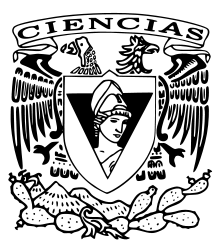
\includegraphics[scale=.29]{img/fciencias1.png}}
	\end{picture}
	
	\begin{center}
		\vspace{-114pt}
		\textbf{\large Matemáticas para las Ciencias II}\\
		\textbf{ Semestre 2020-2}\\
		Prof. Pedro Porras Flores\\
		Ayud. Irving Hernández Rosas \\
		\textbf{Tarea Examen III}\\[0.15cm]
		Kevin Ariel Merino Peña\footnote{Número de cuenta 317031326}\\ [0.12cm]
		\today
	\end{center}
	\vspace{-10pt}
	\rule{19cm}{0.3mm}
	
	\noindent Realice los siguientes ejercicios, escribiendo el procedimiento claramente. Y recuerden la tarea-examen se entregan de manera individual.\\
	
\noindent1.Sea $f: \mathbb{R} \longrightarrow \mathbb{R}$ una función diferenciable. Muestre que $u = f(y - \kappa x)$ es una solución de la ecuación diferencial parcial $$\dfrac{\partial u}{\partial x} + \kappa\dfrac{\partial u}{\partial y} = 0$$
Hagamos una observación sobre $ u $, pues debemos costruir a dicha función con el mismo dominio que f, \textit{i.e. }
\[ u(x,y) = f(y-\kappa x)  \]ahora empleemos la composición de funciones para designar una función auxiliar $ g: \R^2 \to \R $  como sigue $ g(x,y) = y-\kappa x $;
\[ u(x,y) = (f \circ g)(x,y) = f(g(x,y)) \]
luego, tomemos la derivada de $ u $ como 
\[ Du(x,y) = Df(g(x,y)) \]Veamos que, como $ g $ es una función escalar, entonces su derivada es $ \nabla g $ y por la \textbf{regla de la cadena }en funciones compuestas, tenemos que \[ D_u (x,y) = D_f(g(x,y))\nabla g \label{eq:primeraDerivada}\tag{\venus} \]donde $ \nabla g(x,y) = \left( \dfrac{\d g}{\d x}, \dfrac{\d g}{\d y} \right)= \left( -\kappa, 1 \right) $, luego de $ \ref{eq:primeraDerivada} $ tenemos que 
\begin{align*}
	D_u (x,y) &= f'(g(x,y)) \* \left( -\kappa, 1 \right)  && \text{Reemplazando lo que sabemos del gradiente}\\
	D_u (x,y) &= -f'(g(x,y))\kappa, f'(g(x,y)) && \text{Reemplazando lo que sabemos del gradiente}\\
	\dfrac{\d u}{\d x} &= -f'(g(x,y))\kappa  && \text{Derivando con respecto a }x\\
	\dfrac{\d u}{\d y} &= f'(g(x,y)) && \text{Derivando con respecto a }y\\
	\kappa\dfrac{\d u}{\d y} &= f'(g(x,y))\kappa  && \text{Multiplicando ambos miembros por el mismo real }\\
\end{align*}
\[ \dfrac{\partial u}{\partial x} + \kappa\dfrac{\partial u}{\partial y} = -f'(g(x,y))\kappa + f'(g(x,y))\kappa = 0  \]siguiendo la cadena de igualdades, tenemos que 
\[ \dfrac{\partial u}{\partial x} + \kappa\dfrac{\partial u}{\partial y} = 0 \quad \qedsymbol \]

\noindent2.Muestre que si  $u(x,y)$ y $v(x,y)$ tienen segundas parciales mixtas continuas y satisfacen las ecuaciones de 
\begin{subequations}
\label{eq:Maxwell}
Cauchy-Riemann:
\begin{align}
        \dfrac{\partial u}{\partial x} &= \dfrac{\partial v}{\partial y},         \label{eq:MaxB} \\
        \dfrac{\partial u}{\partial y} &= - \dfrac{\partial v}{\partial x}, \label{eq:MaxE}
\end{align}
\end{subequations}

Entonces ambas son armónicas.
\begin{remark}
Una función $u = u(x,y)$ con segundas derivadas parciales continuas que satisface la ecuación de Laplace  $$ \dfrac{\partial^2 u}{\partial x^2} + \dfrac{\partial^2 u}{\partial y^2}= 0,$$ se dice que es una función armónica.
\end{remark}
\noindent Veamos qué ocurre para $ u $ cuando obtenemos sus segundas derivadas
\begin{align*}
	\dfrac{\d^2u}{\d x^2} &= \dfrac{\d}{\d x}\left( \dfrac{\d u}{\d x} \right) &&\text{Por definición de segunda derivada}\\
	\dfrac{\d^2u}{\d x^2} &= \dfrac{\d}{\d x}\left( \dfrac{\d v}{\d x} \right) &&\text{Ya que cumplen las ecuaciones de Cauchy-Riemann}\\
	\dfrac{\d^2u}{\d x^2} &= \dfrac{\d^2 v}{\d x\d y}  &&\text{Volviendo a escribir la ecuación}\\
\end{align*}
por otra parte
\begin{align*}
	\dfrac{\d^2u}{\d y^2} &= \dfrac{\d}{\d y}\left( \dfrac{\d u}{\d y} \right) &&\text{Por definición de segunda derivada}\\
	\dfrac{\d^2u}{\d y^2} &= \dfrac{\d}{\d y}\left( - \dfrac{\d v}{\d x} \right) &&\text{Ya que cumplen las ecuaciones de Cauchy-Riemann}\\
	\dfrac{\d^2u}{\d y^2} &= - \dfrac{\d^2 v}{\d y\d x}&&\text{Reescribiendo}\\
	\dfrac{\d^2u}{\d y^2} &= - \dfrac{\d^2 v}{\d x\d y}&&\text{Ya que por hipótesis $ u $ es de clase }\mathcal{C}^2\\
\end{align*}
de las últimas dos observaciones podemos concluir que
\begin{align*}
	\dfrac{\d^2u}{\d x^2} +\dfrac{\d^2u}{\d y^2} &= \dfrac{\d^2 v}{\d x\d y} +\left( - \dfrac{\d^2 v}{\d x\d y} \right)&&\text{Sumando ambos miembros }\\
	\dfrac{\d^2u}{\d x^2} +\dfrac{\d^2u}{\d y^2} &= 0  &&\text{Así sabemos que $ u $ es armónica}\\
\end{align*}
luego, hagamos algunas observaciones para $ v $

\begin{align*}
\dfrac{\d^2v}{\d x^2} &= \dfrac{\d}{\d x}\left( \dfrac{\d v}{\d x} \right) &&\text{Por definición de segunda derivada}\\
\dfrac{\d^2v}{\d x^2} &= \dfrac{\d}{\d x}\left( - \dfrac{\d u}{\d y} \right) &&\text{Ya que cumplen las ecuaciones de Cauchy-Riemann}\\
\dfrac{\d^2v}{\d x^2} &= - \dfrac{\d^2 u}{\d x\d y}  &&\text{Volviendo a escribir la ecuación}\\
\end{align*}
por otra parte
\begin{align*}
\dfrac{\d^2v}{\d y^2} &= \dfrac{\d}{\d y}\left( \dfrac{\d v}{\d y} \right) &&\text{Por definición de segunda derivada}\\
\dfrac{\d^2v}{\d y^2} &= \dfrac{\d}{\d y}\left(\dfrac{\d u}{\d x} \right) &&\text{Ya que cumplen las ecuaciones de Cauchy-Riemann}\\
\dfrac{\d^2v}{\d y^2} &= \dfrac{\d^2 u}{\d y\d x}&&\text{Reescribiendo}\\
\dfrac{\d^2v}{\d y^2} &=\dfrac{\d^2 u}{\d x\d y}&&\text{Ya que por hipótesis $ v $ es de clase }\mathcal{C}^2\\
\end{align*}
de las últimas dos observaciones podemos concluir que
\begin{align*}
\dfrac{\d^2v}{\d y^2} +\dfrac{\d^2v}{\d x^2} &= \dfrac{\d^2 u}{\d x\d y} +\left( - \dfrac{\d^2 u}{\d x\d y} \right)&&\text{Sumando ambos miembros }\\
\dfrac{\d^2v}{\d y^2} +\dfrac{\d^2v}{\d x^2} &= 0  &&\text{Así sabemos que $ v $ es armónica}\\
\end{align*}
\begin{center}
	$ \therefore $ ambas ecuaciones son armónicas si satisfacen las ecuaciones de  \textit{Cauchy-Riemann} y son de clase $ \mathcal{C}^2 $(que sus segundas derivadas mixtas sean iguales)
\end{center}
\noindent3. Encontrar la expansión a segundo orden de Taylor para $f(x,y) = y^2e^{-x^2}$ en $(1,1)$\\

primero hallemos las derivadas de $ f $
\begin{align*}
	\dfrac{\d}{\d x} \left(y^2 e^{-x^2}\right) &= -2xy^2e^{-x^2} &&\text{Derivando con respecto a }x\\
	\dfrac{\d}{\d y} \left(y^2 e^{-x^2}\right) &= 2ye^{-x^2} &&\text{Derivando con respecto a }y\\
	\dfrac{\d}{\d x} \left(-2xy^2e^{-x^2}\right) &= \left(4x^2 - 2\right)y^2e^{-x^2} &&\text{Derivando con respecto a }xx\\
	\dfrac{\d}{\d y} \left(2y^2e^{-x^2}\right) &= 2e^{-x^2} &&\text{Derivando con respecto a }yy\\
	\dfrac{\d}{\d y} \left(-2xy^2e^{-x^2}\right) &= -4xye^{-x^2} &&\text{Derivando con respecto a }xy, yx\\
\end{align*}
Luego, usando el teorema (visto en clase) sobre la expansión a segundo orden de Taylor para $ x_0 =(1,1) $ está dada por
\begin{align*}
	f(h_1,h_2) &= f(1,1) + h_1f_x(1,1)+ h_2f_y(1,1) + \dfrac{1}{2}\left( h_1^{2}f_{xx}(1,1) + h_1h_2f_{xy}(1,1) + h_1h_2f_{yx}(1,1) + h_2^2f_{yy}(1,1) \right)\\
	f(x,y) &= f(1,1) + xf_x(1,1)+ yf_y(1,1) + \dfrac{1}{2}\left( h_1^2f_{xx}(1,1) + h_1h_2f_{xy}(1,1) + h_1h_2f_{yx}(1,1) + h_2^2f_{yy}(1,1) \right)\\
	f(x,y) &= f(1,1) + x\dfrac{\d f}{\d x}\Bigr|_{(1,1)}+ y\dfrac{\d f}{\d y}\Bigr|_{(1,1)} + \dfrac{1}{2}\left( h_1^2\dfrac{\d^2 f}{\d x^2}\Bigr|_{(1,1)} + h_1h_2\dfrac{\d^2 f}{\d x \d y}\Bigr|_{(1,1)} + h_1h_2\dfrac{\d^2 f}{\d y \d x}\Bigr|_{(1,1)}+ h_2^2\dfrac{\d^2 f}{\d y^2 }\Bigr|_{(1,1)}\right)\\
	f(x,y) &= 1^2e^{-1^2} + x\left( -2xy^2e^{-x^2} \right)\Bigr|_{(1,1)}+ y\dfrac{\d f}{\d y}\Bigr|_{(1,1)} + \dfrac{1}{2}\left( h_1^2\dfrac{\d^2 f}{\d x^2}\Bigr|_{(1,1)} + h_1h_2\dfrac{\d^2 f}{\d x \d y}\Bigr|_{(1,1)} + h_1h_2\dfrac{\d^2 f}{\d y \d x}\Bigr|_{(1,1)}+ h_2^2\dfrac{\d^2 f}{\d y^2 }\Bigr|_{(1,1)}\right)\\
	f(x,y) &= \dfrac{1}{e} -\dfrac{2h_1}{e} + \dfrac{2h_2}{e} + \dfrac{1}{2}\left( h_1^2\dfrac{\d^2 f}{\d x^2}\Bigr|_{(1,1)} + h_1h_2\dfrac{\d^2 f}{\d x \d y}\Bigr|_{(1,1)} + h_1h_2\dfrac{\d^2 f}{\d y \d x}\Bigr|_{(1,1)}+ h_2^2\dfrac{\d^2 f}{\d y^2 }\Bigr|_{(1,1)}\right)\\
	f(x,y) &= \dfrac{1}{e} -\dfrac{2h_1}{e} + \dfrac{2h_2}{e} + \dfrac{1}{2}\left( h_1^2(2e^{-1}) + h_1h_2(-4e^{-1}) + h_1h_2(-4e^{-1}) + h_2^2(2e^{-1})  \right)\\
	f(x,y) &= \dfrac{1}{e} -\dfrac{2h_1}{e} + \dfrac{2h_2}{e} + \dfrac{h_1^2  -4h_1h_2 + h_2^2}{e}\\
	f(x,y) &=  \dfrac{x^2-4xy+y^2+4y-1}{e}\\
\end{align*}

\noindent4. Sea $f: \mathbb{R}^2 \longrightarrow \mathbb{R}$ tal que  $f(x,y) = x^2 - y^2 - xy + 5$. Encuentre los puntos críticos de $f$ y determine si son: mínimos locales, máximos locales o puntos silla.\\
Para ello derivemos la función y localicemos los puntos críticos.

\begin{align*}
	\dfrac{\d f}{\d x} &= \dfrac{\d }{\d x}\left( x^2 - y^2 - xy + 5 \right) &&\text{Derivando con respecto a }x\\
	\dfrac{\d f}{\d x} &= 2x-y &&\text{Aplicando la derivada}\\
	\dfrac{\d f}{\d x} &= -2y-x &&\text{Aplicando la derivada con respecto a $ y $ de }f\\
	\\
	0 &= 2x-y &&\text{Igualemos a }0\\
	0 &= -2y - x &&\text{ }\\
\end{align*}
De la primera ecuación, obtenemos que $ y = 2x $, sustituyendo en la segunda ecuación obtenemos que $ 0 = -5x $, de esta manera sabemos que el único punto crítico que tiene $ f $ es $ (x,y) = (0,0) $. Ahora calculemos las segundas derivadas parciales para conocer el determinante del Hessiano
\begin{align*}
	\dfrac{\d^2 f}{\d x^2} &= 2\\
	\dfrac{\d^2 f}{\d y^2} &= -2\\
	\dfrac{\d^2 f}{\d y \d x} &= -1\\
	\dfrac{\d^2 f}{\d x \d y} &= -1\\
	D\Bigr|_{(0,0)} &= 2 \* (-2) - 1 = -5 < 0\\
\end{align*}
Entonces, usando el teorema visto en clase sobre el determinante del hessiano, ahora sabemos que $ (0,0) $ es un punto silla, es más es el único punto crítico de $ f $.\\


\noindent5. Encuentre los valores máximos y mínimos absolutos de $f(x,y) = x^2 + 3xy + y^2 + 5$ sobre el disco unitario $\mathcal{D} = \{(x,y) \in \mathbb{R}^2 : x^2 + y^2 \leq 1 \}$\\

\noindent Primero calculemos la derivada de $ f $ e igualemos a 0 para encontrar los puntos críticos en el interior del disco.
\begin{align*}
	f_x &= 2x+3y &&\text{Derivando con respecto a }x\\
	f_y &= 2y+3x &&\text{Derivando con respecto a }y\\
	\\
	0 &= 2x+3y &&\text{Igualando a 0 }\\
	0 &= 2y+3x &&\text{Igualando a }0\\
	\\
	4\lambda^2 -8\lambda -5 &= 5 && \text{Ecuación para } \lambda\\
\end{align*}
De lo anterior concluimos que el único punto crítico es $ \vec{x_0} = (0,0) $, además notemos que $ (0,0) \in D $, ahora nombremos la función $ g(x,y) = x^2 + y^2 =1 $, emplearemos multiplicadores de lagrange para resolver
\begin{align*}
	\nabla g &= (2x, 2y) && \text{Calculando el gradiente de }g\\
	\nabla f &= (2x + 3y, 3x + 3y) && \text{Calculando el gradiente de }g\\
	\\
	2x + 3y &= 2x\lambda &&\text{Igualando la primera entrada}\\
	3x + 2y &= 2y\lambda &&\text{Igualando la segunda entrada}\\
	x^2 + y^2 &= 1 &&\text{La restricción dada}\\
\end{align*}
Notemos, de la primera ecuación que $ x \neq 0 $ porque eso implicaría que $ y = 0 $ lo cual no podría pasar por la restricción dada, entonces despejando $ \lambda $ obtenemos que 
\[ \lambda = \dfrac{2x + 3y}{2x} \]
reemplazando en cualquier ecuación obtendremos que $ x^2 = y^2 \implies x = \pm y $, ahora ocupemos esto en la restricción para obtener que 
$ x = \pm \dfrac{\sqrt{2}}{2} $, así tenemos que los puntos críticos son 
\[  \left( \dfrac{\sqrt{2}}{2}, \dfrac{\sqrt{2}}{2} \right), \left( -\dfrac{\sqrt{2}}{2}, \dfrac{\sqrt{2}}{2} \right), \left( \dfrac{\sqrt{2}}{2}, -\dfrac{\sqrt{2}}{2} \right), \left( -\dfrac{\sqrt{2}}{2}, -\dfrac{\sqrt{2}}{2} \right) \]
\begin{align*}
	f \left( \dfrac{\sqrt{2}}{2}, \dfrac{\sqrt{2}}{2} \right) &= 7+ \dfrac{1}{2}\\
	f \left( \dfrac{\sqrt{2}}{2},- \dfrac{\sqrt{2}}{2} \right) &= 4 + \dfrac{1}{2}\\
	f \left( \dfrac{-\sqrt{2}}{2}, \dfrac{\sqrt{2}}{2} \right) &= 4 + \dfrac{1}{2}\\
	f \left( \dfrac{-\sqrt{2}}{2},- \dfrac{\sqrt{2}}{2} \right) &= 7 + \dfrac{1}{2}\\
\end{align*}
por lo tanto, el máximo absoluto es $ 7 + \frac{1}{2} $, en $ \left( -\dfrac{\sqrt{2}}{2},- \dfrac{\sqrt{2}}{2} \right) $ y $ \left( \dfrac{\sqrt{2}}{2}, \dfrac{\sqrt{2}}{2} \right) $.\\
El mínimo absoluto es $ 4 + \frac{1}{2} $, en $ \left( \dfrac{\sqrt{2}}{2},- \dfrac{\sqrt{2}}{2} \right) $ y en $ \left( -\dfrac{\sqrt{2}}{2}, \dfrac{\sqrt{2}}{2} \right) $\\


\noindent6. Suponga que un pentágono está compuesto por un rectángulo coronado por un triángulo isósceles (ver Figura \ref{fig:1}). Si la longitud del perímetro es fija, encuentre el área máxima posible.

\begin{figure}[h]
    \centering
    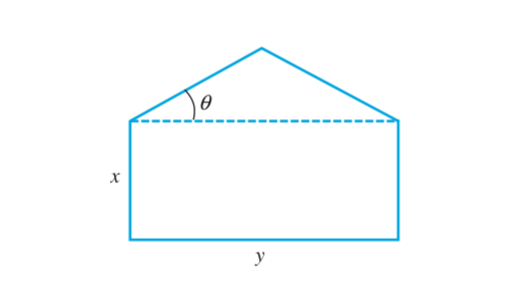
\includegraphics[width=0.5\textwidth]{img/figT}
    \caption{Maximizar el área para un perímetro dado.}
    \label{fig:1}
\end{figure}

Sea $ z $ la longitud de una de los lados del triángulo isóceles sobre el rectángulo en la figura. Sea $ p $ el perímetro del pentágono\[ p = 2x + y + 2z \]
Observemos que 
\begin{align*}
	z \cos(\theta) &= \dfrac{1}{2} y &&\text{Tomando el angulo del la mitad del triangulo iscóceles como referencia}\\
	z  &= \dfrac{y}{2\cos(\theta)} &&\text{Multiplicando ambos lados por } \dfrac{1}{\cos(\theta)} \label{eq:seta} \tag*{\jupiter}\\
	2z  &= \dfrac{y}{\cos(\theta)} &&\text{Multiplicando ambos lados por } 2 \label{eq:dosSeta}\tag*{\mars}\\
\end{align*}

Sea $ a $ el área del pentágono dada por  la suma del rectángulo formado por los lados $ x $, $ y $ y el triángulo superior, entonces 
\begin{align*}
	a &= x\* y + \dfrac{1}{2} yz \sin(\theta) && \text{obteniendo la altura del triangulo con identidades trigonométricas}\\
	a &= xy + \dfrac{y^2\sin(\theta)}{4\cos(\theta)} && \text{Sustituyendo el resultado de }\ref{eq:seta}\\
\end{align*}

Observemos que de esta última ecuación, se nos proporcionan algunas restricciones puesto que el área siempre debe ser positivo y al menos mayor que cero para este ejercicio, por lo que $ 0 < x $, $ 0 < y $ y $ 0 < \theta < \dfrac{\pi}{2} $. Luego, volvamos al perímetro y sustituyamos el valor de $ z $

\begin{align*}
	p &= 2x + y\dfrac{y}{\cos(\theta)} &&\text{Sustituyendo 2z de }\ref{eq:dosSeta}\\
	x &= \dfrac{1}{2}\left( p -y - \dfrac{y}{\cos(\theta)} \right) &&\text{Despejando a }x\\
\end{align*}
Ahora pongamos al área en función de $ y $ y del ángulo

\begin{align*}
	a(y,\theta) &= xy + \dfrac{y^2\sin(\theta)}{4\cos(\theta)} &&\text{De lo construido anteriormente}\\
	a(y,\theta) &= \dfrac{1}{2}py - \dfrac{1}{2}y^2 - \dfrac{y^2}{2\cos(\theta)} + \dfrac{y^2\sin(\theta)}{4\cos(\theta)} &&\text{Sustituyendo el valor de }x\\
\end{align*}

Ahora, al calcular $ \dfrac{\d a}{\d \theta} = 0 $ y $ \dfrac{\d a}{\d y} = 0 $ podemos observar que 
\begin{align*}
	\dfrac{\d a}{\d y} &= \dfrac{p}{2} - y - \dfrac{y}{\cos(\theta)} + \dfrac{y \sin(\theta) }{2 \cos (\theta) }  \\
	0&= \dfrac{p}{2} - y - \dfrac{y}{\cos(\theta)} + \dfrac{y \sin(\theta) }{2 \cos (\theta) }  \\
	\dfrac{p}{2}&=  y \left( 1 + \dfrac{1}{\cos(\theta)} - \dfrac{\sin(\theta)}{2 \cos(\theta)} \right)\\
	\dfrac{p}{2}&=  y \left( \dfrac{2 + 2 \cos(\theta) - \sin(\theta)}{2\cos(\theta)} \right)\\
	y &=  \dfrac{p\cos(\theta)}{2 + 2\cos(\theta) - \sin(\theta
		)}\\
\end{align*}
Por otra parte, buscando los puntos críticos con el ángulo conseguimos lo siquiente:
\begin{align*}
	\dfrac{\d a}{\d \theta} &= - \dfrac{y^2}{2}\left( \dfrac{\sin(\theta)}{\cos^2(\theta)}\right) + \dfrac{y^2}{4}\left(  \dfrac{1}{\cos^2(\theta)} \right) \\
	0 &= - \dfrac{y^2}{2}\left( \dfrac{\sin(\theta)}{\cos^2(\theta)}\right) + \dfrac{y^2}{4}\left(  \dfrac{1}{\cos^2(\theta)} \right) \\
	\dfrac{y^2}{2\cos^2(\theta)}\sin(\theta) &= \dfrac{y^2}{2\cos^2 (\theta)}\* \dfrac{1}{2}\\
	\sin(\theta) &=\dfrac{1}{2}\\
	\theta &=\dfrac{\pi}{6}\\
\end{align*}
Una vez hallado el ángulo, podemos evaluar el coseno en ese punto y sustituirlo en la $ y $, la última ecuación que hayamos para encontrar quién es $ x $
\begin{align*}
	\cos(\dfrac{\pi}{6}) &= \dfrac{\sqrt{3}}{2}\\
	y &=  \dfrac{p\cos(\theta)}{2 + 2\cos(\theta) - \sin(\theta )}\\
	y &=  \dfrac{p\sqrt{3}}{3 + 2\sqrt{3}}\\
\end{align*}
luego, de una ecuación para $ x $
\begin{align*}
	x &= \dfrac{1}{2} \left( p - y - \dfrac{y}{\cos(\theta)} \right)\\
	x &= \dfrac{1}{2} \left( p - \dfrac{p\sqrt{3}}{3 + 2\sqrt{3}} - \dfrac{2p}{3 + 2\sqrt{3}} \right)\\
	x &= \dfrac{p}{2} \left( \dfrac{3 +2\sqrt{3} - \sqrt{3} -2}{3 +2\sqrt{2}} \right)\\
	x &= \dfrac{p(1 + \sqrt{3})}{2(3 + 2\sqrt{3})}\\
\end{align*}
Como ya tenemos quienes son $ x,y $, sustituyamos en la ecuación del área
\begin{align*}
	a\left( \dfrac{p\sqrt{3}}{3 + 2\sqrt{3}},\dfrac{\pi}{6}\right) &= xy + \dfrac{y^2\sin(\theta)}{4\cos(\theta)} \\
	a\left( \dfrac{p\sqrt{3}}{3 + 2\sqrt{3}},\dfrac{\pi}{6}\right) &= \dfrac{p(1 + \sqrt{3})}{2(3 + 2\sqrt{3})}\* \dfrac{p\sqrt{3}}{3 + 2\sqrt{3}} + \dfrac{1}{4}\left(\dfrac{p\sqrt{3}}{3 + 2\sqrt{3}}\right)^2\* \dfrac{\sqrt{3}}{3}\\
	a\left( \dfrac{p\sqrt{3}}{3 + 2\sqrt{3}},\dfrac{\pi}{6}\right) &= \dfrac{p^2 (3 + \sqrt{3})}{2(9 + 12\sqrt{3}+ 12)} + \dfrac{\sqrt{3}}{12}\left( \dfrac{3 p^2}{9 + 12\sqrt{3} + 12} \right)\\
	a\left( \dfrac{p\sqrt{3}}{3 + 2\sqrt{3}},\dfrac{\pi}{6}\right) &= p^2\dfrac{ 18 + 6\sqrt{3} +3 \sqrt{3} }{12(21 + 12\sqrt{3})} \\
	a\left( \dfrac{p\sqrt{3}}{3 + 2\sqrt{3}},\dfrac{\pi}{6}\right) &= p^2\dfrac{ 9 (2 +\sqrt{3})}{12 \* 3 (7 + 4\sqrt{3})} \\
	a\left( \dfrac{p\sqrt{3}}{3 + 2\sqrt{3}},\dfrac{\pi}{6}\right) &= \dfrac{p^2}{4}\*\dfrac{2 + \sqrt{3} }{7 + 4\sqrt{3}} \\
\end{align*}
\begin{center}
	Por lo tanto, el área máxima con un perímetro fijo del pentágono presentado está dado por \[\dfrac{p^2}{4}\*\dfrac{2 + \sqrt{3} }{7 + 4\sqrt{3}}   \]
\end{center}
\noindent7. Analice el comportamiento de las funciones en los puntos indicados. En la parte $b$ el análisis depende de la constante $C$.\\

a) $z = x^2 - y^2 + 3xy $ en $(0,0)$.\\

Para ello calculemos el gradiente de dicha función
\begin{align*}
	\nabla f &= \left( \dfrac{\d }{\d x} (x^2 - y^2 + 3xy),\dfrac{\d }{\d x}   (x^2 - y^2 + 3xy) \right) \\
	\nabla f &= \left( 2x + 3y, -2y + 3x\right) \\
	(0,0) &= \left( 2x + 3y, -2y + 3x\right) \\
	0 &=  2x + 3y \\
	0 &= -2y + 3x \\
\end{align*}
Así podemos concluir que $ (0,0) $ es un punto crítico para nuestra función. Luego calculemos las segundas derivadas parciales para determinal el comportamiento del detnerminante del Hessiano

\begin{align*}
	\dfrac{\d^2 }{\d x^2} f &=  2\\ 
	\dfrac{\d^2 }{\d y^2} f &=  -2\\ 
	\dfrac{\d^2 }{\d xy} f &= 3 = \dfrac{\d^2 }{\d yx} \\
	\\
	D\Bigr|_{(0,0)} &= 2 \* (-2) - 9 = -13 < 0
\end{align*}
\begin{center}
	Así podemos conluir que $ (0,0) $ es un punto silla de $ f $\\
\end{center}

b)  $z = x^2 - y^2 + Cxy $ en $(0,0)$.\\
Para ello tomemos como base el ejercicio anterior y observemos qué ocurre en el determinante del Hessiano, pues 

\[ 	D\Bigr|_{(0,0)} = 2 \* (-2) - C^2 = D < 0 \]
como hay un un signo negativo para el cuadrado de $ C $, siempre se tendrá que no importando el valor de dicha constante siempre será negativo, por lo que siempre será un punto silla :)\\

\noindent8. a) Encuentre la distancia mínima del origen en $\mathbb{R}^2$  a la superficie $z = \sqrt{x^2 - 1}$.\\

Describamos los puntos de la superficie de la siguiente forma 
\[ (x,y, \sqrt{x^2 -1}) \]
Tenemos algunas restricciones para que dicha raíz pueda existir en los reales 
\begin{align*}
	x^2 -1 &\geq 0 \\
	x &\geq 1 \\
	x &\leq -1 \\
\end{align*}
Luego, definamos una función distancia como sigue:
\[  d = \sqrt{x^2 + y^2 + \left(\sqrt{x^2 - 1}\right)^2} \]
\begin{align*}
	d &= \sqrt{x^2 + y^2 + \left(\sqrt{x^2 - 1}\right)^2}\\
	d &= \sqrt{x^2 + y^2 + + x^2 - 1}\\
	d &= \sqrt{2x^2 + y^2 - 1}\\
\end{align*}
Para hacer más sencillas las cuentas, trabajaremos con el cuadrado de $ d $, en clase hicimos lo mismo pues vimos que es válido pues $ d^2 $ tendrá el mismo punto mínimo que $ d $.
Sea $ f := 2x^2 + y^2 -1 $ nuestra función a minimizar. Es fácil observar que para $ y $ no tenemos ninguna restricción dada, por lo que puede ser arbitrario, entonces observemos qué pasa cuando $ y = 0 $, tendríamos que $ f = 2x^2 -1 $ y por una observación que hicimos al principio del ejericicio sabemos que $ x^2 \geq 1 $, así, el minimo valor que tedría nuestra función f sería $ 1 $
pues $ f(\pm1,0) = 2(\pm1)^2-1 = 1 $
\begin{center}
	$ \therefore $ el valor mínimo que tendrá la distancia del origen a la superficie es 1\\
\end{center}

b) Haga lo mismo para la superficie $z = 6xy + 7$\\

Veamos que todos los puntos sobre dicha superficie tendrán la siguiente forma $ (x, y, (6xy + 7)^2)  $, ahora definamos la función distancia como sigue \[ d = \sqrt{x^2 + y^3 + (6xy +7)^2} \]y trabajaremos sin la raíz, por lo que definiremos la función $ f: U \subset \R^2 \to \R $ como $$ f := d^2 =x^2 + y^2 + (6xy + y)^2 $$
\begin{align*}
	f(x,y) &= x^2 + y^2 + (6xy + y)^2 \\
	f(x,y) &= x^2 + y^2 + 6^2x^2y^2 +2\*6xy\*7 +7^2 \\
	f(x,y) &= 36x^2y^2  + x^2 + y^2 + 48xy + 49 \\
\end{align*}
Veamos que en el caso hipotético de que $ x^2 + y^2 = 0 $ el valor más bajo que $ f(x,y) $ tendría es $ 49 $, por lo tanto, la distancia mínima es $ 7 $, pero derivemos para encontrar los demás puntos críticos.
\begin{align*}
	\dfrac{\d f}{\d x} &= 36x^2y^2  + x^2 + y^2 + 48xy + 49\\
	\dfrac{\d f}{\d x} &= 72xy^2+2x+84y\\
	\\
	\dfrac{\d f}{\d y} &= 36x^2y^2  + x^2 + y^2 + 48xy + 49\\
	\dfrac{\d f}{\d y} &= 72x^2 y + 2y + 84x\\
\end{align*}
ahora igualemos amboas ecuaciones a 0 y obtengamos
\begin{align*}
	72x^2 y + 2y + 84x &= 0\\
	 72xy^2+2x+84y &= 0 \\
	72x^2 y + 2y + 84x - (72xy^2+2x+84y) &= 0\\
	72xy ( x - y ) + 82x - 82y &= 0\\
	( x - y ) (72xy + 82) &= 0\\
\end{align*}
Como el producto de dos reales es cero y si y sólo si algunos de los dos es cero, entonces
\[ x = y \lor 72xy = -82 \]
Sustituyamos la priera ecuación en $ \dfrac{\d f}{\d x} $
\begin{align*}
	\dfrac{\d f}{\d x} &= 72xx^2 + 2x + 84x\\
	\dfrac{\d f}{\d x} &= x(72x^2 + 84)\\
	0 &= x(72x^2 + 84)\\
\end{align*}
debido a que $72x^2 + 84   $ siempre será positivo en la última ecuación, entonces $ x = 0 = y $ y si sustituimos en la ecuación que se nos proporcinó al principio del problema, obtendremos que 
\[ z = 6 \* 0 \* 0 + 7 \implies z = 7 \]entonces el punto crítico que hallamos es $ (0,0,7) $ lo que nos regala $ d = \sqrt{0^2 + 0^2+ 7^2 } = 7 $.\\

Ahora veamos qué ocurre con $ xy = -\dfrac{41}{36} $ y sustituyamos en la ecuación del problema $ z = 6 (-\dfrac{41}{36}) + 7 \implies \dfrac{-41}{6} + \dfrac{42}{6} = \dfrac{1}{6} $ de $ xy = -\dfrac{41}{36} $ despejemos a x para usar $ x = -\dfrac{41}{36y} $
\begin{align*}
	\dfrac{\d f}{\d x} &= 72xy^2 + 2x + 84y\\
	\dfrac{\d f}{\d x} &= 72\left(\dfrac{-41}{36y}\right)y^2 + 2\left( -\dfrac{41}{36y} \right) + 84y\\
	\dfrac{\d f}{\d x} &= -82y - \dfrac{82}{36y}+ 84y\\
	0 &= 2y -\dfrac{82}{36y}\\
	2y &= \dfrac{41}{18y}\\
	36y^2 &= 41\\
	y &= \sqrt{\dfrac{41}{36}}\\
	y &= \dfrac{\sqrt{41}}{6}\\
\end{align*}
Sistituyamos en $ x = -\dfrac{41}{36y} $
\begin{align*}
	x &= -\dfrac{41}{36y}\\
	x &= -\dfrac{41}{36 \* \frac{\sqrt{41}}{6}} \\
	x &= -\dfrac{\sqrt{41}}{6}\\
\end{align*}
Con ambos valores sólo basta calcular $ z $ en la ec. del ejecicio
\[ z = 6 \* \dfrac{\sqrt{41}}{6} \* (- \dfrac{\sqrt{41}}{6}) + 7 = \dfrac{41}{6} + \dfrac{42}{6} = \dfrac{1}{6}  \]
Ahora susituyamos en la ecuación de la distancia

\begin{align*}
	d &= \sqrt{x^2 +y^2 + z^2}\\
	d &= \sqrt{(-\dfrac{\sqrt{41}}{6})^2 +(\dfrac{\sqrt{41}}{6})^2 + (\dfrac{1}{6})^2}\\
	d &= \sqrt{\dfrac{41}{36} + \dfrac{41}{36} + \dfrac{1}{6} }\\
	d &= \dfrac{83}{6}\\
\end{align*}
Entre nuestos dos puntos hallados $ \dfrac{83}{6} $ es el mínimo :)\\



\noindent9. Encuentre los puntos y valores críticos de las siguientes funciones sujetas a las restricciones:\\


a) $f(x,y) = x^2 - 2xy + 2y^2$, restringido a $x^2 + y^2 =1$.\\

b) $f(x,y) = \cos{(x^2 - y^2)}{}$, restringido a $x^2 + y^2 =1$.\\

c) $f(x,y) = \dfrac{x^2 - y^2}{x^2 + y^2}$, restringido a $x + y =1$.\\

d) $f(x,y) = \cos^2{x} +\cos^2{y}$, restringido a $x + y =\frac{\pi}{4}$.


\noindent10. Encuentre el máximo de la función $f(x,y) = xy$ sobre la curva $(x +1)^2 + y^2 =1$, definamo suna función $ g: U \subset \R^2 \to \R $ como $ g(x,y) = (x +1)^2 + y^2 = 1$

\[ \nabla g = (x-1, 2y) \]
\begin{align*}
	\dfrac{\d f}{\d x} &= y = \lambda \dfrac{\d g}{\d x}\\
	y &= \lambda(x - 1) \\
	\dfrac{\d f}{\d y} &= x = \lambda \dfrac{\d g}{\d y}\\
	x &=  \lambda 2y\\
	\\
	g(x,y) &= 1\\
	(x +1)^2 + y^2 &= 1
\end{align*}
luego, despejemos $ x,y $, de
\begin{align*}
	x &= 2y \lambda  & y &= \dfrac{x}{2\lambda} & \lambda &= \dfrac{x}{2y}  \\
\end{align*}
\begin{align*}
	y &= (2x + 2)\lambda\\
	y &= (2x + 2)(\frac{x}{2y})\\
	2y^2 &= 2x^2 + 2x\\
	0 &= 2x^2 + 2x - 2y^2\\
	0 &= x^2 + x - y^2 \label{eq:unoDiez}\tag{10a} \\
\end{align*}
de la restricción podemos ver que 
\begin{align*}
	(x +1)^2 + y^2 &= 1\\
	x^2 + 2x+ 1+ y^2 &= 1\\
	x^2 + 2x+ y^2 &= 0 \label{eq:dosDiez}\tag{10b} \\
\end{align*}
Si resolvemos $ \ref{eq:unoDiez} $ y $ \ref{eq:dosDiez} $ 
\begin{align*}
	x^2 + x - y^2 &= 0\\
	x^2 + 2x+ y^2 &= 0\\
	2x^2 + 3x &= 0\\
	x(2x + 3) &= 0\\
	\\
	x_1 &= 0\\
	x_2 &= \dfrac{-3}{2}\\
\end{align*}
Si sustituimos en $ x = 2\lambda y $ obtendremos que si $ x = 0 $ entonces $ y = 0 $, y si $ x = -\dfrac{3}{2} $ entonces $ y = \pm \dfrac{\sqrt{3}}{2} $ ( de $x^2 + y^2 +2x = 0  $)

Entonces tenemos lo siguientes puntos

\[ (0,0), \left(-\dfrac{3}{2}, - \dfrac{\sqrt{3}}{2}\right), \left(-\dfrac{3}{2},  \dfrac{\sqrt{3}}{2}\right) \]
Evaluemos en todos ellos
\begin{align*}
	f(0,0) &= xy = 0\\ 
	f\left(-\dfrac{3}{2}, - \dfrac{\sqrt{3}}{2}\right) &= xy = \dfrac{3\sqrt{3}}{4}\\ 
	f\left(-\dfrac{3}{2},  \dfrac{\sqrt{3}}{2}\right) &= xy = -\dfrac{3\sqrt{3}}{4}\\ 
\end{align*}
Podemos concluir que el máximo valor es $ \dfrac{3\sqrt{3}}{4} $ \\

\noindent11. Encuentre la distancia más cercana del punto $(a_1, a_2, a_3) \in \mathbb{R}^3$ al plano cuya ecuación está dada por: $b_1x_1 + b_2x_2 + b_3x_3 + b_0 = 0$, donde $(b_1, b_2, b_3) \neq 0 $\\

Sea $ D(x_1,x_2,x_3) = (x_1 - a_1)^2 + (x_2 - a_2)^2 + (x_3 - a_3)^2 $ sujeto a la restricción $ g(x_1, y_1, z_1) = b_1x_1 + b_2x_2 + b_3 x_3 + b_0 = 0$ con $ (b_1, b_2, b_3) \neq 0  $. Calculemos el gradiente de $ D $ y $ g $
\begin{align*}
	\nabla D(x_1, x_2, x_2) &= (2x_1 - 2a_1, 2x_2 - 2a_2, 2x_3 - 2a_3)\\
	\nabla g(x_1, x_2, x_2) &= (b_1, b_2, b_3) \neq (0,0,0)\\
\end{align*}
Ahora podemos obtener las siguientes ecuaciones
\begin{align*}
	\lambda b_1 &= 2x_1 - 2a_1 \\
	\lambda b_2 &= 2x_2 - 2a_2 \\
	\lambda b_3 &= 2x_3 - 2a_3 \\
	0 &= b_1x_1 + b_2x_2 + b_3x_3 + b_0 \\
\end{align*}
Para ello emplearemos el método de \textit{Gauss-Jordan}
\begin{align*}
	\begin{pmatrix}
	2 & 0 & 0 & -b_1 \\
	0 & 2 & 0 & -b_2 \\
	0 & 0 & 2 & -b_3 \\
	b_1 & b_2 & b_3 & 0 \\
	\end{pmatrix} \* \begin{pmatrix}
	x_1\\
	x_2\\
	x_3\\
	\lambda\\
	\end{pmatrix} &= \begin{pmatrix}
	2a_1\\
	2a_2\\
	2a_3\\
	-b_0\\
	\end{pmatrix}\\
	\begin{pmatrix}
	2 & 0 & 0 & -b_1 \\
	0 & 2 & 0 & -b_2 \\
	0 & 0 & 2 & -b_3 \\
	0 & b_2 & b_3 & \frac{b_1^2}{2} \\
	\end{pmatrix} \* \begin{pmatrix}
	x_1\\
	x_2\\
	x_3\\
	\lambda\\
	\end{pmatrix} &= \begin{pmatrix}
	2a_1\\
	2a_2\\
	2a_3\\
	-b_0 - b_1a_1\\
	\end{pmatrix}\\ %%%
	\begin{pmatrix}
	2 & 0 & 0 & -b_1 \\
	0 & 2 & 0 & -b_2 \\
	0 & 0 & 2 & -b_3 \\
	0 & 0 & b_3 & \frac{b_1^2}{2} + \frac{b_2^2}{2} \\
	\end{pmatrix} \* \begin{pmatrix}
	x_1\\
	x_2\\
	x_3\\
	\lambda\\
	\end{pmatrix} &= \begin{pmatrix}
	2a_1\\
	2a_2\\
	2a_3\\
	-b_0 - b_1a_1 - b_2a_2\\
	\end{pmatrix}\\ %%
	\begin{pmatrix}
	2 & 0 & 0 & -b_1 \\
	0 & 2 & 0 & -b_2 \\
	0 & 0 & 2 & -b_3 \\
	0 & 0 & 0 & \frac{b_1^2}{2} + \frac{b_2^2}{2} + \frac{b_3^2}{2} \\
	\end{pmatrix} \* \begin{pmatrix}
	x_1\\
	x_2\\
	x_3\\
	\lambda\\
	\end{pmatrix} &= \begin{pmatrix}
	2a_1\\
	2a_2\\
	2a_3\\
	-b_0 - b_1a_1 - b_2a_2 - b_3a_3\\
	\end{pmatrix}\\ %%
\end{align*}
si despejamos lambda de la última fila $ \therefore \lambda = \dfrac{-2(b_0 + b_1 a_1 + b_2 a_2 + b_3 a_3)}{b_1^2 + b_2^2 + b_3^2} $
\begin{align*}
	2x_3 - b_3 \lambda &= 2a_3\\
	x_3 &= \dfrac{2a_3 + b_3 \lambda}{2} \\
	\\
	2x_2 - b_2 \lambda &= 2a_2\\
	x_2 &= \dfrac{2a_2 + b_2 \lambda}{2} \\
	\\
	2x_1 - b_1 \lambda &= 2a_1\\
	x_1 &= \dfrac{2a_1 + b_1 \lambda}{2} \\
\end{align*}
Ahora, veamos el hessiano de la función
\begin{align*}
	\dfrac{\d^2 D}{\d x_1^2} &= 2\\
	\dfrac{\d^2 D}{\d x_2^2} &= 2\\
	\dfrac{\d^2 D}{\d x_3^2} &= 2\\
	\dfrac{\d^2 D}{\d x_1x_2} &= 0\\
	\dfrac{\d^2 D}{\d x_2x_3} &= 0\\
	\dfrac{\d^2 D}{\d x_1x_3} &= 0\\
\end{align*}
entonces el arreglo quedaría 
\begin{align*}
	HD(x_1,x_2,x_3) &= \begin{bmatrix}
	2 & 0 & 0\\
	0 & 2 & 0\\
	0 & 0 & 2\\
	\end{bmatrix}
\end{align*}
Así que $ H_1 = \abs{2} > 0 $, $ H_2 = \begin{vmatrix}
	2 & 0\\
	0 & 2\\
\end{vmatrix}  = 4 > 0$ y finalmente $ H_3 = \begin{vmatrix}
	2 & 0 & 0\\
	0 & 2 & 0\\
	0 & 0 & 2\\
\end{vmatrix} = 8 > 0$, eso nos permite concluir que el punto crítico en cuestíon es un mínimo local, ahora evaluemos

\begin{align*}
	D\left( \dfrac{2a_1 + b_1\lambda}{2}, \dfrac{2a_2 + b_2 \lambda}{2}, \dfrac{2a_3 + b_3 \lambda}{2} \right) &= \left( \dfrac{2a_1 + b_1\lambda}{2} - a_1 \right)^2 + \left( \dfrac{2a_2 + b_2 \lambda}{2} - a_2 \right)^2 + \left( \dfrac{2a_3 + b_3 \lambda}{2} - a_3 \right)^2\\
	D\left( \dfrac{2a_1 + b_1\lambda}{2}, \dfrac{2a_2 + b_2 \lambda}{2}, \dfrac{2a_3 + b_3 \lambda}{2} \right) &= \left( \dfrac{b_1\lambda}{2}  \right)^2 + \left( \dfrac{b_2 \lambda}{2} \right)^2 + \left( \dfrac{b_3 \lambda}{2}\right)^2\\
	D\left( \dfrac{2a_1 + b_1\lambda}{2}, \dfrac{2a_2 + b_2 \lambda}{2}, \dfrac{2a_3 + b_3 \lambda}{2} \right) &= \dfrac{\lambda^2}{4}\left( b_1^2 + b_2^2 + b_3^2 \right)\\
\end{align*}
luego, podemos emplear que $ \lambda = \dfrac{-2(b_0 + a_1b_1 +a_2 b_2 + a_2 b_3)}{b_1^2 + b_2^2 + b_3^2} $

\[ 	D\left( \dfrac{2a_1 + b_1\lambda}{2}, \dfrac{2a_2 + b_2 \lambda}{2}, \dfrac{2a_3 + b_3 \lambda}{2} \right) = \dfrac{(b_0 + a_1 b_1 + a_2 b_2 + a_3 b_3)^2}{b_1^2 + b_2^2 + b_3^2} \]
\begin{center}
	Como habiamos tomado a D como la función distnacia pero al cuadrado ahora podemos ver que la \textbf{mínima} distnacia está dada por
	\[ \sqrt{	D\left( \dfrac{2a_1 + b_1\lambda}{2}, \dfrac{2a_2 + b_2 \lambda}{2}, \dfrac{2a_3 + b_3 \lambda}{2} \right)} = \dfrac{|b_0 + a_1 b_1 + a_2 b_2 + a_3 b_3|}{\sqrt{b_1^2 + b_2^2 + b_3^2}}  \]
\end{center}


\noindent12. Encuentre el punto sobre la linea de intersección de los planos  $a_1x_1 + a_2x_2 + a_3x_3 = 0$ y $b_1x_1 + b_2x_2 + b_3x_3 + b_0 = 0$ que es más cercano al origen.

Sean $ \vec{a}  = (a_1, a_2, b_2)$ y $ \vec{b} = (b_1, b_2, b_3) $ los vectores de la distancia, tomemos una función $ D $ como el cuadrado de la distancia (para no trabajar con raices) 
\begin{align*}
	D(x_1, x_2, x_3) &= (x_1 -0)^2 + (x_2 -0)^2 + (x_3 -0)^2\\
	D(x_1, x_2, x_3) &= x_1^2 + x_2^2 + x_3^2\\
\end{align*}
Sujetas a las siguientes restricciones 
\begin{align*}
	g_1(x_1, x_2, x_3) &= a_1 x_2 + a_2 x_2 + a_3 x_3 = 0\\
	g_2(x_1, x_2, x_3) &= b_1 x_2 + b_2 x_2 + b_3 x_3  + b_0 = 0\\
\end{align*}
Primero supongamos que $ \nabla g_1 \neq 0 $ y $ \nabla g_2 \neq 0 $ entonces
\begin{align*}
	\nabla D &= (2x_1, 2x_2, 2x_3)\\
	\nabla g_1 &= (a_1, a_2, a_3)\\
	\nabla g_2 &= (b_1, b_2, b_3)\\
\end{align*}
Así se nos permite plantear el siguiente sistema de ecuaciones
\setcounter{equation}{0}
\begin{align} 
	2x_1 &= \l_1 a_1 + \l_2 b_1\\
	2x_2 &= \l_1 a_2 + \l_2 b_2\\
	2x_3 &= \l_1 a_3 + \l_2 b_3\\
	a_1 x_1 + a_2 x_2 + a_3 x_3 &= 0\\
	b_1 x_1 + b_2 x_2 + b_3 x_3 &= -b_0
\end{align}
resolvamos por el método de \textit{Gauss-Jordan}
\begin{align*}
	\begin{pmatrix}
	2 & 0 & 0 & -a_1 & -b_1\\
	0 & 2 & 0 & -a_2 & -b_2\\
	0 & 0 & 2 & -a_3 & -b_3\\
	a_1 & a_2 & a_3 & 0 & 0\\
	b_1 & b_2 & b_3 & 0 & 0\\
	\end{pmatrix}\begin{pmatrix}
	x_1\\
	x_2\\
	x_3\\
	\l_1\\
	\l_2\\
	\end{pmatrix} &= \begin{pmatrix}
	0\\
	0\\
	0\\
	0\\
	-b_0\\
	\end{pmatrix}\\%%
	\begin{pmatrix}
	2 & 0 & 0 & -a_1 & -b_1\\
	0 & 2 & 0 & -a_2 & -b_2\\
	0 & 0 & 2 & -a_3 & -b_3\\
	a_1 & a_2 & a_3 & 0 & 0\\
	b_1 & b_2 & b_3 & 0 & 0\\
	\end{pmatrix} &= 	\begin{pmatrix}
	2 & 0 & 0 & -a_1 & -b_1\\
	0 & 2 & 0 & -a_2 & -b_2\\
	0 & 0 & 2 & -a_3 & -b_3\\
	0 & a_2 & a_3 & \frac{a_1^2}{2} & \frac{a_1b_1}{2}\\
	0 & b_2 & b_3 & \frac{a_1b_1}{2} & \frac{b_1^2}{2}\\
	\end{pmatrix}\\ %%
	\begin{pmatrix}
	2 & 0 & 0 & -a_1 & -b_1\\
	0 & 2 & 0 & -a_2 & -b_2\\
	0 & 0 & 2 & -a_3 & -b_3\\
	0 & a_2 & a_3 & \frac{a_1^2}{2} & \frac{a_1b_1}{2}\\
	0 & b_2 & b_3 & \frac{a_1b_1}{2} & \frac{b_1^2}{2}\\
	\end{pmatrix} &= \begin{pmatrix}
	2 & 0 & 0 & -a_1 & -b_1\\
	0 & 2 & 0 & -a_2 & -b_2\\
	0 & 0 & 2 & -a_3 & -b_3\\
	0 & 0 & a_3 & \frac{(a_1^2 + a_2^2)}{2} & \frac{(a_1b_1 + a_2b_2)}{2}\\
	0 & 0 & b_3 & \frac{(a_1b_1 + a_2b_2)}{2} & \frac{(b_1^2 + b_2^2)}{2}\\
	\end{pmatrix}
\end{align*}
\begin{align*}
	\begin{pmatrix}
	2 & 0 & 0 & -a_1 & -b_1\\
	0 & 2 & 0 & -a_2 & -b_2\\
	0 & 0 & 2 & -a_3 & -b_3\\
	0 & 0 & a_3 & \frac{(a_1^2 + a_2^2)}{2} & \frac{(a_1b_1 + a_2b_2)}{2}\\
	0 & 0 & b_3 & \frac{(a_1b_1 + a_2b_2)}{2} & \frac{(b_1^2 + b_2^2)}{2}\\
	\end{pmatrix} &= \begin{pmatrix}
	2 & 0 & 0 & -a_1 & -b_1\\
	0 & 2 & 0 & -a_2 & -b_2\\
	0 & 0 & 2 & -a_3 & -b_3\\
	0 & 0 & 0 & \frac{(a_1^2 + a_2^2 + a_3^2)}{2} & \frac{(a_1b_1 + a_2b_2 + a_3 b_3)}{2}\\
	0 & 0 & 0 & \frac{(a_1b_1 + a_2b_2 + a_3 b_3)}{2} & \frac{(b_1^2 + b_2^2 + b_3^2)}{2}\\
	\end{pmatrix}\\ %%
	\begin{pmatrix}
	2 & 0 & 0 & -a_1 & -b_1\\
	0 & 2 & 0 & -a_2 & -b_2\\
	0 & 0 & 2 & -a_3 & -b_3\\
	0 & 0 & 0 & \frac{(a_1^2 + a_2^2 + a_3^2)}{2} & \frac{(a_1b_1 + a_2b_2 + a_3 b_3)}{2}\\
	0 & 0 & 0 & \frac{(a_1b_1 + a_2b_2 + a_3 b_3)}{2} & \frac{(b_1^2 + b_2^2 + b_3^2)}{2}\\
	\end{pmatrix} &= \begin{pmatrix}
	2 & 0 & 0 & -a_1 & -b_1\\
	0 & 2 & 0 & -a_2 & -b_2\\
	0 & 0 & 2 & -a_3 & -b_3\\
	0 & 0 & 0 & \frac{(a_1^2 + a_2^2 + a_3^2)}{2} & \frac{(a_1b_1 + a_2b_2 + a_3 b_3)}{2}\\
	0 & 0 & 0 & 0 & \frac{(b_1^2 + b_2^2 + b_3^2)}{2} - \dfrac{(a_1b_2 + a_2 b_2 + a_3 b_3)^2}{2(a_1^2 + a_2^2 + a_3^2)}\\
	\end{pmatrix} \begin{pmatrix}
	x_1\\
	x_2\\
	x_3\\
	\l_1\\
	\l_2\\
	\end{pmatrix}
\end{align*}
entonces tenemos que 
\setcounter{equation}{0}
\begin{align}
	2x_1 - \l_1 a_1 - \l_2 b_1 &= 0\\
	2x_2 - \l_1 a_2 - \l_2 b_2 &= 0\\
	2x_3 - \l_1 a_3 - \l_2 b_3 &= 0\\
	\left( \dfrac{a_1^2 + a_2^2 + a_3^2}{2} \right)\l_1 + \dfrac{(a_1 b_1 + a_2 b_2 + a_3 b_3)}{2}\l_2 &= 0\\
	\dfrac{(b_1^2 + b_2^2 + b_3^2 )}{2} \l_2 - \dfrac{(a_1 b_2 + a_2 b_2 + a_3 b_3)^2}{2(a_1^2 + a_2^2 + a_3^2)}\l_2 &= -b_0 
\end{align}
Observemos que si asumimos a $ b_0 = 0 $ entonces en $ (5) $ tendríamos que $ \l_2 = 0 $, también por $ (4) $, $ \lambda_1 = 0 $ y así sabríamos que por $ (1),(2),(3) $ $ x_1 = x_2 = x_3 = 0 $ lo que significaría que $ (0,0,0) $ es la interseccion de los planos y además es la distancia más cercana al origen. Entonces asumamos que $ b_0 \neq 0 $ entonces $ \l_2 \neq 0 $, reescribamos $ (4) $ y $ (5) $ para hacerlos más claros

\begin{align*}
	(\vec{a} \* \vec{a}) \l_1 + (\vec{a} \* \vec{b}) \l_2 &= 0 \label{eq:penUltima}\tag{4}\\
	\frac{\l_2}{2}\left( \vec{b}\* \vec{b} - \dfrac{(\vec{a} \* \vec{b})^2}{\vec{a} \* \vec{a}} \right) &= -b_0 \label{eq:Ultima}\tag{5}
\end{align*}
\end{document}
